%% DONE
\id{МРНТИ 28.17.19}{https://doi.org/10.58805/kazutb.v.1.26-903}

\begin{articleheader}
\sectionwithauthors{А.Д. Бургегулов, Ш.А. Джомартова, Ә.Т. Мазакова, М.С. Әлиасқар, Т.Ж. Мазаков, А.Д. Майлыбаева}{ПОСТРОЕНИЕ ПУТЕЙ ЭВАКУАЦИИ ЛЮДЕЙ ИЗ МНОГОЭТАЖНОГО ЗДАНИЯ ПРИ УГРОЗЕ И ВОЗНИКНОВЕНИИ ПОЖАРА}

{\bfseries \textsuperscript{1}А.Д. Бургегулов\alink{https://orcid.org/0000-0003-3019-3352},
\textsuperscript{1}Ш.А. Джомартова\textsuperscript{\envelope } \alink{https://orcid.org/0000-0002-5882-5588},
\textsuperscript{1}Ә.Т. Мазакова\alink{https://orcid.org/0000-0003-4904-3557},
\textsuperscript{2} М.С. Әлиасқар\alink{https://orcid.org/0000-0002-3013-6617},
\textsuperscript{1,2}Т.Ж. Мазаков\alink{https://orcid.org/0000-0001-9345-5167},
\textsuperscript{3}А.Д. Майлыбаева\alink{https://orcid.org/0009-0000-2958-1935}}
\end{articleheader}

\begin{affiliation}
\emph{¹Казахский национальный университет имени аль-Фараби, Алматы, Казахстан,}

\emph{\textsuperscript{2}Международный инженерно-технологический университет, Алматы, Казахстан,}

\emph{\textsuperscript{3}Атырауский университет имени Х. Досмухамедова, Атырау, Казахстан}

\raggedright \textsuperscript{\envelope }{\em Корреспондент-автор: \href{mailto:jomartova@mail.ru}{\nolinkurl{jomartova@mail.ru}}}
\end{affiliation}

Статья посвящена разработке алгоритма для построения эвакуационных
маршрутов в случае чрезвычайных ситуаций, таких как пожар. Разработанный
алгоритм используется в качестве математической модели интеллектуальной
системы противопожарной безопасности и реализован на языке Python. Его
эффективность подтверждается на примере модельной задачи, демонстрируя
возможности мониторинга и реагирования на возникновение пожара.

Созданный алгоритм оптимизации маршрутов эвакуации основан на решении
транспортных задач, обладает высокой универсальностью и легко
адаптируется к практическим требованиям оперативного и безопасного
выхода людей из здания. В статье представлены результаты численного
моделирования, а также рассмотрены перспективы дальнейшего развития
подобных систем.

Разработанные алгоритмы могут быть применены не только при пожаре, но и
в случае других чрезвычайных ситуаций, таких как наводнения или
землетрясения, что позволяет минимизировать риски и снизить ущерб от
катастроф.

{\bfseries Ключевые слова:} интеллектуальная система, противопожарная
безопасность, транспортная задача, пожар, чрезвычайная ситуация,
эвакуация.

\begin{articleheader}
{\bfseries ӨРТ ҚАУПІ ТӨНГЕН НЕМЕСЕ ПАЙДА БОЛҒАН ЖАҒДАЙДА КӨПҚАБАТТЫ ҮЙЛЕРДЕН АДАМДАРДЫ ЭВАКУАЦИЯЛАУ ЖОЛДАРЫН САЛУ}

{\bfseries \textsuperscript{1}А.Д. Бургегулов,
\textsuperscript{1}Ш.А. Джомартова\textsuperscript{\envelope },
\textsuperscript{1}Ә.Т. Мазақова,
\textsuperscript{2} М.С. Әлиасқар,
\textsuperscript{1,2}Т.Ж. Мазақов,
\textsuperscript{3}А.Д.~Майлыбаева}
\end{articleheader}

\begin{affiliation}
\emph{\textsuperscript{1}Әл-Фараби атындағы Қазақ ұлттық университеті, Алматы, Қазақстан,}

\emph{\textsuperscript{2}Халықаралық инженерлік және технология университеті, Алматы, Қазақстан,}

\emph{\textsuperscript{3} Х.Досмұхамедов атындағы Атырау университеті, Атырау, Қазақстан,}

\emph{e-mail: \href{mailto:jomartova@mail.ru}{\nolinkurl{jomartova@mail.ru}}}
\end{affiliation}

Мақала өрт сияқты төтенше жағдайлар кезінде эвакуациялау жолдарын құру
алгоритмін әзірлеуге арналған. Әзірленген алгоритм өрт қауіпсіздігінің
интеллектуалды жүйесінің математикалық моделі ретінде пайдаланылады және
Python тілінде жүзеге асырылады. Оның тиімділігі өрттің пайда болуын
бақылау және әрекет ету мүмкіндіктерін көрсете отырып, мысал ретінде
үлгілік мәселені қолдану арқылы расталады.

Эвакуациялау жолдарын оңтайландырудың құрылған алгоритмі көлік
мәселелерін шешуге негізделген, өте әмбебап және адамдардың ғимараттан
тез және қауіпсіз шығуының практикалық талаптарына оңай бейімделуі
мүмкін. Мақалада сандық модельдеу нәтижелері берілген, сондай-ақ мұндай
жүйелерді одан әрі дамыту перспективалары қарастырылған.

Әзірленген алгоритмдер тек өрт кезінде ғана емес, сонымен қатар су
тасқыны немесе жер сілкінісі сияқты басқа да төтенше жағдайлар кезінде
де қолданылуы мүмкін, бұл тәуекелдерді барынша азайтуға және апаттардан
келетін шығынды азайтуға мүмкіндік береді.

{\bfseries Түйін сөздер:} интеллектуалды жүйе, өрт қауіпсіздігі, көлік
тапсырмасы, өрт, төтенше жағдай, эвакуация.

\begin{articleheader}
{\bfseries CONSTRUCTION OF EVACUATION ROUTES FOR PEOPLE FROM A MULTI-STORY BUILDING IN CASE OF A THREAT OR OCCURRENCE OF A FIRE}

{\bfseries
\textsuperscript{1}A.D. Burgegulov,
\textsuperscript{1}Sh.A. Jomartova\textsuperscript{\envelope },
\textsuperscript{1}A.T. Mazakova,
\textsuperscript{2}M.S. Aliaskar,
\textsuperscript{1,2}T.Zh. Mazakov,
\textsuperscript{3}A.D.~Mailybayeva}
\end{articleheader}

\begin{affiliation}
\emph{\textsuperscript{1}Kazakh National University named after Al-Farabi, Almaty, Kazakhstan,}

\emph{\textsuperscript{2}International Engineering and Technology University, Almaty, Kazakhstan,}

\emph{\textsuperscript{3}Atyrau University named after Kh. Dosmukhambetov, Atyrau, Kazakhstan,}

\emph{e-mail: \href{mailto:jomartova@mail.ru}{\nolinkurl{jomartova@mail.ru}}}
\end{affiliation}

The article is devoted to the development of an algorithm for
constructing evacuation routes in case of emergency situations, such as
fire. The developed algorithm is used as a mathematical model of an
intelligent fire safety system and is implemented in Python. Its
effectiveness is confirmed by the example of a model problem,
demonstrating the capabilities of monitoring and responding to a fire.

The created algorithm for optimizing evacuation routes is based on
solving transport problems, is highly versatile and easily adapts to the
practical requirements of prompt and safe exit of people from a
building. The article presents the results of numerical modeling, and
also considers the prospects for further \\development of such systems.

The developed algorithms can be applied not only in case of fire, but
also in case of other emergency situations, such as floods or
earthquakes, which allows to minimize risks and reduce damage from
disasters.

{\bfseries Keywords:} intelligent system, fire safety, transport task, fire,
emergency, evacuation

\begin{multicols}{2}
{\bfseries Введение.} Пожары представляют собой одни из наиболее
разрушительных природных явлений, способных причинить значительный и
зачастую необратимый вред экосистемам нашей планеты. В условиях быстрого
научно-технического прогресса риски, связанные с пожарами, возрастают
из-за усложнения технологических систем, развития электротехнической
отрасли, широкого использования углеводородных материалов и влияния
социально-экономических факторов. Все эти элементы в совокупности
повышают вероятность возникновения аварий и катастроф, что приводит к
серьезным экономическим и социальным последствиям.

Дополнительные трудности возникают из-за эксплуатации устаревших систем
противопожарной безопасности, которые не соответствуют современным
стандартам. Также важным аспектом является отсутствие комплексного
подхода к решению данной проблемы на уровне государства.

В условиях крупных многоэтажных зданий и комплексов, где сосредоточено
большое количество людей, быстрое и эффективное реагирование на угрозу
пожара становится критически важным. Очевидно, что традиционные методы и
технологии уже не способны обеспечить необходимый уровень безопасности.

{\bfseries Материалы и методы.} Разработка специальных методов и
вычислительных алгоритмов и программно-аппаратных комплексов,
позволяющих в реальном времени предупреждать, строить оптимальные
маршруты при возникновении ЧС являются актуальной проблемой {[}1-3{]}.
Транспортная задача может быть применена для оптимального распределения
людей по выходам в процессе эвакуации из здания, с целью сокращения
времени эвакуации и предотвращения скопления людей.

\emph{1. Постановка задачи}

Для разработки математической модели маршрутов эвакуации из здания
введем следующие обозначения:

\(m\) - количество этажей в здании;

\(n_{i}\) - количество кабинетов на \(i\)- м этаже,
\(i = \overline{1,m}\) ;

\(k_{i}\) - количество лестниц и выходов на \(i\)- м этаже,
\(i = \overline{1,m}\) ;

\(a_{ij}\) - количество людей в \(j\)- м кабинете на \(i\)- м этаже,
\(i = \overline{1,m}\) , \(j = \overline{1,n_{i}}\);

\(b_{ij}\) - проходимость \(j\)- й лестницы (выхода) на \(i\)- м этаже,
\(i = \overline{1,m}\) , \(j = \overline{1,k_{i}}\),

\(x_{ij}^{p}\) - количество людей из эвакуируемых из \(i\)- го кабинета
через \(j\)- ю лестницу (выход) на \(p\)- м этаже,
\(i = \overline{1,n_{p}}\) , \(j = \overline{1,k_{p}}\),
\(p = \overline{1,m}\),

\(c_{ij}^{p}\) - время (или расстояние) необходимое для перемещения
человека из \(i\)- го кабинета через \(j\)- ю лестницу (выход) на \(p\)-
м этаже, \(i = \overline{1,n_{p}}\) , \(j = \overline{1,k_{p}}\),
\(p = \overline{1,m}\).

Создадим формализованную математическую модель, которая будет
соответствовать определенным требованиям для организации эвакуации
людей.

1) все люди должны покинуть каждый этаж здания

\begin{equation}
\sum_{j = 1}^{n_{i}}x_{ij}^{p} = a_{pi},i = \overline{1,n_{p}},p = \overline{1,m}
\end{equation}

2) пропускная способность выходов не должна быть превышена (не создавалась давка):

\begin{equation}
\sum_{j = 1}^{n_{i}}x_{ij}^{p} = b_{pi},i = \overline{1,k_{p}},p = \overline{1,m}
\end{equation}

3) условие неотрицательности переменных

\begin{equation}
x_{ij}^{p} \geq 0,\quad i = \overline{1,n_{p}},\quad j = \overline{1,k_{p}},\quad p = \overline{1,m},
\end{equation}

4) общее время эвакуации должно быть минимальным

\begin{equation}
Z = \sum_{p = 1}^{m}{\sum_{i = 1}^{n_{p}}{\sum_{j = 1}^{k_{p}}{c_{ij}^{p}x_{ij}^{p} \rightarrow \min}}}.
\end{equation}

2. \emph{Теоретическая часть}

Существует множество методов для решения транспортной задачи (1)-(4). В
дальнейшем мы рассмотрим метод потенциалов.

{\bfseries Лемма 1.} Сложность метода потенциалов для задачи (1)-(4) может
быть оценена следующим образом {[}4{]}.

\begin{equation}
O(\sum_{i = 1}^{p}n_{i} \ast \sum_{i = 1}^{p}k_{i} \ast (\sum_{i = 1}^{p}n_{i} + \sum_{i = 1}^{p}{k_{i}))}
\end{equation}

{\bfseries Лемма 2.} Пусть имеются две числовые неотрицательные
последовательности \(a_{i}\) и \(b_{i}\) , \(i = \overline{1,n}\). Тогда
справедливо следующее нераенство {[}5-7{]}

\begin{equation}
\max_{i = 1,n}{(a}_{i} + b_{i}) \leq \max_{i = 1,n}a_{i} + \max_{i = 1,n}b_{i}
\end{equation}

Предлагается модификация транспортной задачи, адаптированная к проблеме
эвакуации людей из многоэтажного здания.

На первом этапе решается транспортная задача для верхнего этажа, с целью
минимизации функционала

\begin{equation}
Z_{m} = \sum_{i = 1}^{n_{m}}{\sum_{j = 1}^{k_{m}}{c_{ij}^{m}x_{ij}^{m} \rightarrow \min}}
\end{equation}

при ограничениях
\begin{equation}
\begin{aligned}
    \sum_{j = 1}^{n_{i}}x_{ij}^{m} &= a_{mi}, \quad i = \overline{1,n_{m}}, \\
    \sum_{j = 1}^{n_{i}}x_{ij}^{m} &= b_{mi}, \quad i = \overline{1,k_{p}}, \\
    x_{ij}^{m} &\geq 0, \quad i = \overline{1,n_{m}}, \quad j = \overline{1,k_{m}}
\end{aligned}
\end{equation}

Обозначим через s -- номер шага итерации. Пусть s =1.

Шаг S. s=s+1. Если s=m то переходи к шагу N.

После выполнения предыдущего этапа становится известно, сколько людей
спустилось с верхнего этажа по каждой лестнице. Введем фиктивные
кабинеты, которые будут представлять собой лестницы, соединяющие
исследуемый этаж с предыдущим. Количество людей в фиктивном кабинете
будет определяться на основе предыдущего решения.

В результате передем к следующей транспортной задаче

минимизировать функционал

\begin{equation}
Z_{s} = \sum_{i = 1}^{n_{s}}{\sum_{j = 1}^{k_{s}}{c_{ij}^{s}x_{ij}^{s} \rightarrow \min}}
\end{equation}

при ограничениях

\begin{equation}
\begin{aligned}
\sum_{j = 1}^{n_{i}}x_{ij}^{s} &= a_{si},i = \overline{1,n_{s}}, \\
\sum_{j = 1}^{n_{i}}x_{ij}^{s} &= b_{s - 1,i},i = \overline{n_{s},n_{s} + k_{s - 1}}, \\
\sum_{j = 1}^{n_{i}}x_{ij}^{s} &= b_{mi},i = \overline{1,k_{s}}, \\
x_{ij}^{s} \geq 0,\quad i &= \overline{1,n_{s} + k_{s - 1}},\quad j = \overline{1,k_{m}}.
\end{aligned}
\end{equation}

Возвращаемся к шагу S.

Шаг N. Полученные на предыдущих шагах решения \(x_{ij}^{s} \geq 0\) ,
\(i = \overline{1,n_{s}}\) , \(s = \overline{1,m}\), и составляют план
эвакуации из многоэтажного здания.

Введем обозначение

\begin{equation}
k_{0} = 0
\end{equation}

{\bfseries Теорема.} Сложность предложенного метода для задачи (1)-(4)
имеет следующую оценку

\begin{equation}
O(m \ast \max_{i = 1,p}k_{i} \ast {(\max_{i = 1,p}n_{i} + \max_{i = 1,p}k_{i})}^{2})
\end{equation}

{\bfseries Доказательство.}

\[m \ast \max_{i = 1,p}{(n}_{i} + k_{i - 1}) \ast \max_{i = 1,p}k_{i} \ast \left( \max_{i = 1,p}n_{i} + \max_{i = 1,p}k_{i} \right)\]

\[O(m \ast \max_{i = 1,p}{(n}_{i} + k_{i - 1}) \ast \max_{i = 1,p}k_{i} \ast (\max_{i = 1,p}n_{i} + \max_{i = 1,p}k_{i}))\]

3. \emph{{\bfseries Программная реализация}}

Исходные данные о здании извлекаются из текстового файла Fzdan.txt,
первая строка которого содержит целое число, обозначающее:

- Ne - количество этажей.

В последующих строках представлена информация о количестве кабинетов и
лестниц (выходов), ведущих вниз (или из здания):

- Nk - количество кабинетов,

- Nl - количество лестниц (выходов).

Данные о кабинетах здания берутся из текстового файла Fkabn.txt, где
построчно указаны:

- этаж, на котором расположен кабинет,

- номер кабинета,

- максимальное количество людей, которые могут находиться в кабинете.

Информация о лестницах здания содержится в текстовом файле Flest.txt, в
котором построчно указаны:

- этаж, на котором он находится,

- номер лестницы,

- пропускная способность лестницы.

В текстовом файле Fsvja.txt описаны взаимосвязи между кабинетами,
лестницами и выходами. Каждая строка включает следующие данные:

- первый объект,

- второй объект, с которым он связан,

- тип связи (1 - между кабинетом и лестницей, 2 - между лестницами),

- расстояние между объектами в метрах или время, необходимое для
преодоления расстояния.

4. \emph{{\bfseries Экспериментальная часть}}

Для иллюстрации возможностей разработанного алгоритма были выполнены
расчеты в рамках следующей модельной задачи.

Здание состоит из четырех этажей. На первом этаже размещены четыре
кабинета и предусмотрены четыре выхода на улицу. На втором и третьем
этажах также находятся по четыре кабинета, а количество лестниц, ведущих
на нижний этаж, составляет три. Четвертый этаж включает три кабинета и
две лестницы, ведущие на третий этаж.

Для определения оптимальных маршрутов эвакуации использованы методы
решения транспортных задач {[}8-9{]}.

Программа сохраняет результаты численных расчетов в текстовом файле и
визуализирует их в виде графа. Это позволяет наглядно представить
оптимальные маршруты эвакуации и структуру взаимосвязей между элементами
здания.

На основе предоставленных данных создается граф, где вершины
K\textsubscript{i} обозначают кабинеты, а вершины L\textsubscript{i} --
лестницы и выходы.
\end{multicols}

\begin{figure}[H]
	\centering
	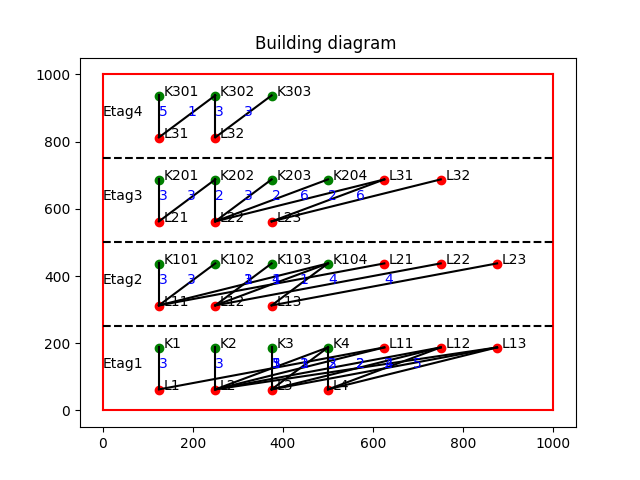
\includegraphics[width=0.6\textwidth]{media/ict2/image7}
	\caption*{Рис.1 - Экран с визуализацией полученного графа}
\end{figure}

\begin{multicols}{2}
На рисунке 1 кабинеты обозначены зеленым кругом, лестницы и выходы --
красным.

Связи между объектами представлены стрелками: кабинет-лестница,
лестница-лестница. Количество людей, эвакуируемых через соответствующую
лестницу, отображается синим цветом.

{\bfseries Выводы.} В данной статье были проанализированы основные аспекты
проектирования и создания интеллектуальной централизованной
противопожарной системы безопасности для умных городов. После изучения
существующих традиционных систем и выявления их недостатков, мы перешли
к рассмотрению инновационных решений, включая применение искусственного
интеллекта и машинного обучения, а также их интеграцию с другими
компонентами умного города.

Современная версия системы успешно справляется с задачей определения и
оптимизации маршрутов эвакуации, принимая во внимание характеристики
здания и распределение людей. Тем не менее, существуют определенные
ограничения, связанные с фиксированностью входных данных. В частности,
система не учитывает динамические изменения в конфигурации здания, такие
как временное закрытие или блокировка отдельных выходов. Это сказывается
на актуальности некоторых эвакуационных сценариев в реальных условиях.
Для преодоления этих ограничений и расширения функциональности системы
предлагается интеграция датчиков, способных передавать информацию о
состоянии выходов и других ключевых элементов здания в режиме реального
времени.

В заключение следует подчеркнуть, что интеллектуальные системы
противопожарной безопасности, развиваясь и интегрируясь в инфраструктуру
умных городов, открывают новые горизонты для повышения безопасности и
снижения рисков для жизни и здоровья граждан. Однако их успешное
внедрение требует глубокого анализа и учета множества факторов, а также
тесного сотрудничества между технологическими компаниями, научными
учреждениями и городскими властями. Кроме того, такие системы должны
функционировать в рамках единой городской управленческой структуры,
объединяя данные и функции с другими подсистемами, такими как
экологический мониторинг, транспортные системы и управление зданиями.
Использование отдельных сенсоров и актуальных данных позволит создать
более гибкую и адаптивную систему, способную оперативно реагировать на
изменения ситуации и определять наиболее безопасные и эффективные
маршруты эвакуации.

Искусственный интеллект и машинное обучение могут быть применены для
постоянного совершенствования алгоритмов и моделей, основанных на
собственном опыте компании и данных из реальной жизни. Это позволит
разрабатывать более точные прогнозы и предлагать рекомендации по
повышению общей безопасности зданий. Система может расширить свои
возможности, создав мобильное приложение для информирования граждан и
координации их действий. Это будет способствовать формированию единого
информационного пространства, в котором все участники процесса, от
спасателей до обычных граждан, смогут получать актуальную информацию и
действовать более эффективно. Технология дополненной реальности может
быть использована для моделирования следов на месте происшествия и
других визуальных данных {[}10{]}.

Предложенные методы и подходы имеют значительный потенциал в области
защиты от природных катастроф, управления массовыми мероприятиями и в
других сферах, где требуется быстрое и эффективное реагирование на
изменения обстановки. {[}11-13{]}.

\emph{{\bfseries Финансирование.}Работа выполнена за счет средств НИИ
математики и механики при КазНУ имени аль-Фараби и грантового
финансирования научных исследований на 2023--2025 годы по проекту
AP19678157.}
\end{multicols}

\begin{center}
{\bfseries Литература}
\end{center}

\begin{references}
1. Пирогов Н.С. Анализ причин пожаров в зданиях культурно-досугового
значения. // Пожарный надзор. -- 2023.- №1. - С.67-73.

2. Смирнов В.П. Прогнозирование путей эвакуации при пожаре в общественных
зданиях // \\Авт.доктор.дисс. спец. 05.26.03, 2018. - 50 с.

3. Иванов П.Н. Исследование времени блокирования путей эвакуации
токсичными продуктами горения на промышленных объектах //Авт.канд.дисс.
спец. 05.26.03, 2019.30 с.

4. Кормен, Томас X. и др. А45 Алгоритмы: Построение и анализ, 3-е изд.:
Пер. с англ. -М.: ООО ``И. Д. Вильямс'', 2013.-1328 с. ISBN
978-5-8459-1794-2

5. \href{https://www.researchgate.net/profile/Derek-Clements-Croome}{Derek
John Clements-Croome} Intelligent Buildings: Design Management and
Operation- ICE Publishing, 2004.-408 p. ISBN 0 7277 3266 8

6. Бургегулов А.Д., Мазаков Т.Ж., Зиятбекова Г.З., Саметова А.А.,
Джолдасова Б.У. Применение интеллектуальных систем пожарной безопасности
в умных городах // Вестник КазУТБ.- 2023. - № 2(19). - С. 7-20. DOI
10.58805/kazutb.v.2.19-84

7. Жадан В. Г. Методы оптимизации. Часть II. Численные алгоритмы:
учебное пособие / В. Г. Жадан. - М. : МФТИ, 2015. - 320 с. ISBN
978-5-7417 (Ч. II)

8. Рафгарден
Т\href{https://www.meloman.kz/other/rafgarden-t-sovershennyj-algoritm-grafovye-algoritmy-i-struktury-dannyh.html?srsltid=AfmBOoonzl3DLF5EZHXaStUKbeOPMt0iOX2nrgpmPI-HIND3-7hOvRYs}{.}:
Совершенный алгоритм. Графовые алгоритмы и структуры данных. -- Питер:
Питер-Трейд, 2020. - 340 с. ISBN 978-5-4461-1272-2

9. Сесекин А. Н.,~Ченцов А. А.,~Ченцов А. Г. Задачи маршрутизации
перемещений. -- Мз-во ``Лань'', 2022. - 240 с. ISBN 978-5-8114-9999-1

10. Paes D., Feng Zh., King M., Shad H.K., Sasikumar P., Pujoni D.,
Lovreglio R. Optical see-through augmented reality fire safety training
for building occupants //Automation in Construction. - 2024.-Vol.162. -
ISSN 0926-5805. DOI
\href{https://doi.org/10.1016/j.autcon.2024.105371}{10.1016/j.autcon.2024.105371}

11. Krichen M., Abdalzaher M.S., Elwekeil M., Fouda M.M. Managing
natural disasters: An analysis of technological advancements,
opportunities, and challenges //Internet of Things and Cyber-Physical
Systems.- 2024.-Vol.4.- P.99-109, ISSN 2667-3452.

\href{https://doi.org/10.1016/j.iotcps.2023.09.002}{DOI
10.1016/j.iotcps.2023.09.002}

12. Мазаков Т.Ж., Бургегулов А.Д., Джомартова Ш.А., Мазакова А.Т.,
Саметова А.А., Досаналиева А.Т. Построение маршрутов для эвакуации
сотрудников из здания при возникновении чрезвычайной ситуации // Вестник
КазУТБ.- 2024.- № 1(22).- С.68-74

DOI 10.58805/kazutb.v.1.22-292

13. Бургегулов А., Зиятбекова Г., Мазаков Т., Саметова А., Алиаскар М.
Использование технологий Интернета вещей для предотвращения пожаров //
Международная конференция по электротехнике и информационным технологиям
(ICEF 2023), Алматы, 2023. С.349-355
\end{references}

\begin{center}
{\bfseries References}
\end{center}

\begin{references}
1. Pirogov N.S. Analiz prichin pozharov v zdanijah
kul' turno-dosugovogo znachenija. // Pozharnyj nadzor.
-2023.- №1. - S.67-73.{[}in Russian{]}

2. Smirnov V.P. Prognozirovanie putej jevakuacii pri pozhare v
obshhestvennyh zdanijah // Avt.doktor.diss. spec. 05.26.03, 2018. - 50
s. {[}in Russian{]}

3. Ivanov P.N. Issledovanie vremeni blokirovanija putej jevakuacii
toksichnymi produktami gorenija na promyshlennyh ob\#ektah
//Avt.kand.diss. spec. 05.26.03, 2019.30 s. {[}in Russian{]}

4. Kormen, Tomas X. i dr. A45 Algoritmy: Postroenie i analiz, 3-e izd.:
Per. s angl. -M.: OOO ``I. D. Vil' jams'', 2013.-1328 s.
ISBN 978-5-8459-1794-2{[}in Russian{]}

5. \href{https://www.researchgate.net/profile/Derek-Clements-Croome}{Derek
John Clements-Croome} Intelligent Buildings: Design Management and
Operation- ICE Publishing, 2004.-408 p. ISBN 0 7277 3266 8

6. Burgegulov A.D., Mazakov T.Zh., Zijatbekova G.Z., Sametova A.A.,
Dzholdasova B.U. Primenenie intellektual' nyh sistem
pozharnoj bezopasnosti v umnyh gorodah // Vestnik KazUTB.- 2023. - №
2(19). - S. 7-20. DOI 10.58805/kazutb.v.2.19-84. {[}in Russian{]}

7. Zhadan V. G. Metody optimizacii. Chast'{} II.
Chislennye algoritmy: uchebnoe posobie / V. G. Zhadan. - M. : MFTI,
2015. - 320 s. ISBN 978-5-7417 (Ch. II). {[}in Russian{]}

8. Rafgarden T.: Sovershennyj algoritm. Grafovye algoritmy i struktury
dannyh. -- Piter: Piter-Trejd, 2020. - 340 s. ISBN 978-5-4461-1272-2.
{[}in Russian{]}

9. Sesekin A. N., Chencov A. A., Chencov A. G. Zadachi marshrutizacii
peremeshhenij. -- Mz-vo ``Lan''', 2022. - 240 s. ISBN
978-5-8114-9999-1. {[}in Russian{]}

10. Paes D., Feng Zh., King M., Shad H.K., Sasikumar P., Pujoni D.,
Lovreglio R. Optical see-through augmented reality fire safety training
for building occupants //Automation in Construction. - 2024.-Vol.162. -
ISSN 0926-5805. DOI
\href{https://doi.org/10.1016/j.autcon.2024.105371}{10.1016/j.autcon.2024.105371}

11. Krichen M., Abdalzaher M.S., Elwekeil M., Fouda M.M. Managing
natural disasters: An analysis of technological advancements,
opportunities, and challenges //Internet of Things and Cyber-Physical
Systems.- 2024.-Vol.4.- P.99-109, ISSN 2667-3452.
\href{https://doi.org/10.1016/j.iotcps.2023.09.002}{DOI
10.1016/j.iotcps.2023.09.002}

12. Mazakov T.Zh., Burgegulov A.D., Dzhomartova Sh.A., Mazakova A.T.,
Sametova A.A., Dosanalieva A.T. Postroenie marshrutov dlja jevakuacii
sotrudnikov iz zdanija pri vozniknovenii chrezvychajnoj situacii //
Vestnik KazUTB.- 2024.- № 1(22).- S.68-74
DOI 10.58805/kazutb.v.1.22-292. {[}in Russian{]}

13. Burgegulov A., Zijatbekova G., Mazakov T., Sametova A., Aliaskar M.
Ispol' zovanie tehnologij Interneta veshhej dlja
predotvrashhenija pozharov // Mezhdunarodnaja konferencija po
jelektrotehnike i informacionnym tehnologijam (ICEF 2023), Almaty, 2023.
S.349-355. {[}in Russian{]}
\end{references}

\begin{authorinfo}
\emph{{\bfseries Сведения об авторах}}

Бургегулов А.Д.- докторант КазНУ им.аль-Фараби, Алматы, Казахстан,
e-mail: \href{mailto:dizel_kz@bk.ru}{\nolinkurl{dizel\_kz@bk.ru}};

Джомартова Ш.А. - доктор технических наук, доцент, КазНУ им. аль-Фараби,
Алматы, Казахстан, e-mail:\\
\href{mailto:jomartova@mail.ru}{\nolinkurl{jomartova@mail.ru}};

Мазақова Ә.Т.- докторант КазНУ им.аль-Фараби, Алматы, Казахстан, e-mail:
\href{mailto:aigerym97@mail.ru}{\nolinkurl{aigerym97@mail.ru}};

Әлиасқар М.С. - старший преподаватель МИТУ, Алматы, Казахстан, e-mail:
\href{mailto:m.alyasqar@gmail.ru}{\nolinkurl{m.alyasqar@gmail.ru}};

Мазаков Т.Ж. - доктор физико-математических наук, профессор, КазНУ им.
аль-Фараби, Алматы, Казахстан, e-mail:
\href{mailto:tmazakov@mail.ru}{\nolinkurl{tmazakov@mail.ru}};

Майлыбаева А.Д. -- к.ф.-м.н., доцент кафедры «Информатика» Атырауского
универститета имени Х. Досмухамедова, Атырау, Казахстан, e-mail:
\href{mailto:a.maylibayeva@asu.edu.kz}{\nolinkurl{a.maylibayeva@asu.edu.kz}}

\emph{{\bfseries Information about the author}}

Burgegulov A.D. - Doctoral student of Al-Farabi Kazakh National
University, Almaty, Kazakhstan, e-mail:
\href{mailto:dizel_kz@bk.ru}{\nolinkurl{dizel\_kz@bk.ru}};

Jomartova Sh.A. - Doctor of Technical Sciences, Associate Professor,
Al-Farabi KazNU, Almaty, Kazakhstan, e-mail:\\
\href{mailto:jomartova@mail.ru}{\nolinkurl{jomartova@mail.ru}};

Mazakova A.T.- Doctoral student of Al-Farabi Kazakh National University,
Almaty, Kazakhstan, e-mail:
\href{mailto:aigerym97@mail.ru}{\nolinkurl{aigerym97@mail.ru}};

Aliaskar M.S. - Senior Lecturer, MITU, Almaty, Kazakhstan, e-mail:
\href{mailto:m.alyasqar@gmail.ru}{\nolinkurl{m.alyasqar@gmail.ru}};

Mazakov T.Zh. - Doctor of Physical and Mathematical Sciences, Professor,
Al-Farabi KazNU, Almaty, Kazakhstan, e-mail:
\href{mailto:tmazakov@mail.ru}{\nolinkurl{tmazakov@mail.ru}};

Mailybayeva A.D. - PhD, Associate Professor, Department of Computer
Science, Atyrau University named after Kh. \\Dosmukhambetov, Atyrau,
Kazakhstan, e-mail:
\href{mailto:a.maylibayeva@asu.edu.kz}{\nolinkurl{a.maylibayeva@asu.edu.kz}}
\end{authorinfo}
